\begin{frame}
    \frametitle{Temario para estas slides}
    
    \begin{itemize}
        \item Graph-SLAM / Factor Graph
        \item Loop-Closure
        \item Bundle Adjustment
    \end{itemize}
    
\end{frame}

\begin{frame}
    \frametitle{¿Qué es SLAM?}
    
    Para que un robot móvil pueda navegar de manera autónoma es necesario que conozca su ubicación y cuente con una representación del entorno donde se encuentra. Estos problemas se conocen como el problema Localización y el problema de Mapeo. En el caso más general, donde no se cuenta con un la localización del robot ni con un mapa a priori del entorno, dichas problemas se abordan de manera simultánea. Esto da origen al problema de SLAM (\emph{Simultaneous Localizacion and Mapping}).
    \begin{block}{}
        SLAM es el problema de resolver la localización y el mapeo al mismo tiempo.
    \end{block}
    
\end{frame}


\begin{frame}
    \frametitle{Ejemplo de SLAM}
    
    \begin{figure}
        \subfloat[Realidad]
        {
            \fbox{\includegraphics[width=0.44\textwidth]{slam_example_gt1.pdf}}
        }\hfill{}
        \subfloat[Sistema de SLAM del robot]
        {
            \fbox{\includegraphics[width=0.44\textwidth]{slam_example_robot1.pdf}}
        }
    \end{figure}
    
\end{frame}

\begin{frame}
    \frametitle{Ejemplo de SLAM}

    \begin{figure}
        \subfloat[Realidad]
        {
            \fbox{\includegraphics[width=0.44\textwidth]{slam_example_gt2.pdf}}
        }\hfill{}
        \subfloat[Sistema de SLAM del robot]
        {
            \fbox{\includegraphics[width=0.44\textwidth]{slam_example_robot2.pdf}}
        }
    \end{figure}
    
\end{frame}

\begin{frame}
    \frametitle{Ejemplo de SLAM}
    
    \begin{figure}
        \subfloat[Realidad]
        {
            \fbox{\includegraphics[width=0.44\textwidth]{slam_example_gt3.pdf}}
        }\hfill{}
        \subfloat[Sistema de SLAM del robot]
        {
            \fbox{\includegraphics[width=0.44\textwidth]{slam_example_robot3.pdf}}
        }
    \end{figure}
    
\end{frame}

\begin{frame}
    \frametitle{Ejemplo de SLAM}
    
    \begin{figure}
        \subfloat[Realidad]
        {
            \fbox{\includegraphics[width=0.44\textwidth]{slam_example_gt4.pdf}}
        }\hfill{}
        \subfloat[Sistema de SLAM del robot]
        {
            \fbox{\includegraphics[width=0.44\textwidth]{slam_example_robot4.pdf}}
        }
    \end{figure}
    
\end{frame}

\begin{frame}
    \frametitle{Ejemplo de SLAM}
    
    \begin{figure}
        \subfloat[Realidad]
        {
            \fbox{\includegraphics[width=0.44\textwidth]{slam_example_gt5.pdf}}
        }\hfill{}
        \subfloat[Sistema de SLAM del robot]
        {
            \fbox{\includegraphics[width=0.44\textwidth]{slam_example_robot5.pdf}}
        }
    \end{figure}
    
\end{frame}

\begin{frame}
    \frametitle{Ejemplo de SLAM}
    
    \begin{figure}
        \subfloat[Realidad]
        {
            \fbox{\includegraphics[width=0.44\textwidth]{slam_example_gt6.pdf}}
        }\hfill{}
        \subfloat[Sistema de SLAM del robot]
        {
            \fbox{\includegraphics[width=0.44\textwidth]{slam_example_robot6.pdf}}
        }
    \end{figure}
    
\end{frame}

\begin{frame}
    \frametitle{Ejemplo de SLAM}
    
    \begin{figure}
        \subfloat[Realidad]
        {
            \fbox{\includegraphics[width=0.44\textwidth]{slam_example_gt7.pdf}}
        }\hfill{}
        \subfloat[Sistema de SLAM del robot]
        {
            \fbox{\includegraphics[width=0.44\textwidth]{slam_example_robot7.pdf}}
        }
    \end{figure}
    
\end{frame}

\begin{frame}
    \frametitle{Ejemplo de SLAM}
    
    \begin{figure}
        \subfloat[Realidad]
        {
            \fbox{\includegraphics[width=0.44\textwidth]{slam_example_gt8.pdf}}
        }\hfill{}
        \subfloat[Sistema de SLAM del robot]
        {
            \fbox{\includegraphics[width=0.44\textwidth]{slam_example_robot8.pdf}}
        }
    \end{figure}
    
\end{frame}

\begin{frame}
    \frametitle{Aquitectura general de SLAM}
    
    \begin{figure}[!h]
            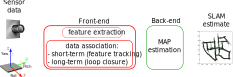
\includegraphics[width=\textwidth]{images/slam_frontend_backend.pdf}
    \end{figure}
    
\end{frame}

\begin{frame}
    \frametitle{Tipos de SLAM Back-ends}
    \note{Información extraída de https://youtu.be/BuRCJ2fegcc y de https://youtu.be/Alu59K8zvYs}
    \footnotesize
    \begin{itemize}
        \item Basados en Kalman Filter (EKF-SLAM)
        \item Basados en Particle Filter (FastSLAM, Rao-Blackwellized Particle Filter, Gmapping)
        \item Basados en Least-Squares (Graph-SLAM, Bundle Adjustment)
        \begin{itemize}
            \item Pose-Graph (solo contiene las poses del robot, el mapa es marginalizado\footnote{Marginalizar es el proceso de remover variables sin perder información.})
            \item Factor-Graph (contiene poses y landmarks)
        \end{itemize}
            Herramientas de optimización
            \begin{itemize}
            \item Ceres
            \item GTSAM
            \item g2o
            \end{itemize}
    \end{itemize}

    \begin{center}
        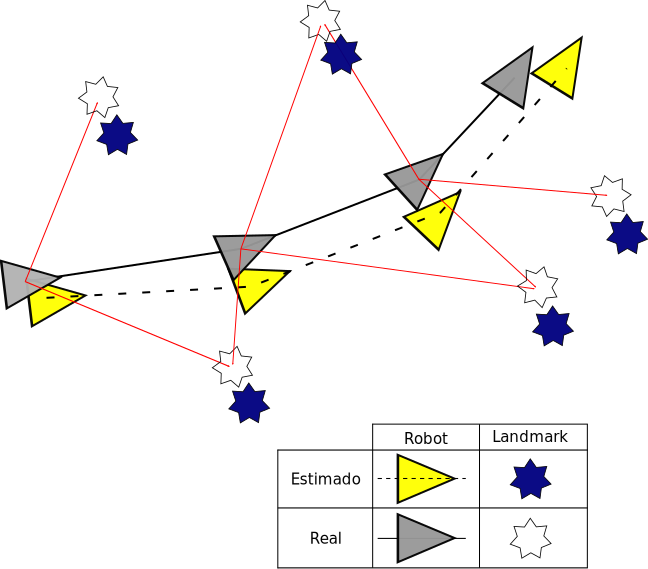
\includegraphics[width=0.25\textwidth]{images/slam-landmarks.pdf}
    \end{center}
    
\end{frame}